\Chapter{RÉSULTAT}\label{sec:Theme2}

Les résultats sont présentés en commençant d’abord par décrire l’implémentation du modèle conceptuel d’automate présenté dans la sous-section~\ref{subsection_cadre_conceptuel}. Ensuite, ce sera présenté successivement les résultats propres à chacun des sous-objectifs décrits dans le chapitre~\ref{chapitre_methode}.

\section{Implémentation: du modèle conceptuel au modèle opérationnel}

L’implémentation de la machine (conceptuelle) est passée par la programmation manuelle d’une première interface et d’un premier noyau, en mettant à jour une version préliminaire de générateur basé sur une GUI\cite{bluiksnot_repo} en lui intégrant la capacité de générer du code à partir d’un module externe via son «hook» au moment de l’installation. La version à ce jour, ainsi que ses guides d’utilisation et ses scripts associés, sont disponibles sur le site de ERPLibre\footnote{\url{https://erplibre.ca}}.

L’interface permet l’interactivité avec un utilisateur ou le système-cible. L’interface est découplée en deux ensembles de méta-données: µ$_C^A$ et µ$_C^B$. µ$_C^B$ est l’ensemble qui paramétrise le passage de méta-données au code pour un module spécifique. µ$_C^A$ est l’ensemble qui paramétrise le passage de code aux méta-données tout en préparant un µ$_C^B$ adapté à ce module spécifique. Ce découplage a permis l’adaptation de l’interface au contexte de l’installation de modules sur une instance Odoo via des «hooks». Par la suite, un ensemble supplémentaire de méta-données, noté µ$_C^0$, a été dégagé de la programmation manuelle de versions successives de µ$_C^A$. µ$_C^0$ sert à initialiser une version de départ de µ$_C^A$.

Le noyau prend les paramètres issus de l’interface pour créer des méta-données, générer l’ensemble des fichiers des modules désirés (mode direct) et faire de la rétro-ingénierie (mode indirect) sur des modules existants.

\subsection{Développement et amélioration continue}

Dans la figure~\ref{fig:dia_sequence_gc}, µ$_C^0$, µ$_C^A$, µ$_C^B$, C et M sont tous des modules installables sur Odoo. $M^i$ et $M^d$ sont des sections de code dans le module M. µ$_C^0$, µ$_C^A$ et µ$_C^B$ dépendent de M. µ$_C^A$, c’est les macro-méta-données, que µ$_C^B$, c’est les micro-méta-données.

\begin{figure}[htb]
\centering
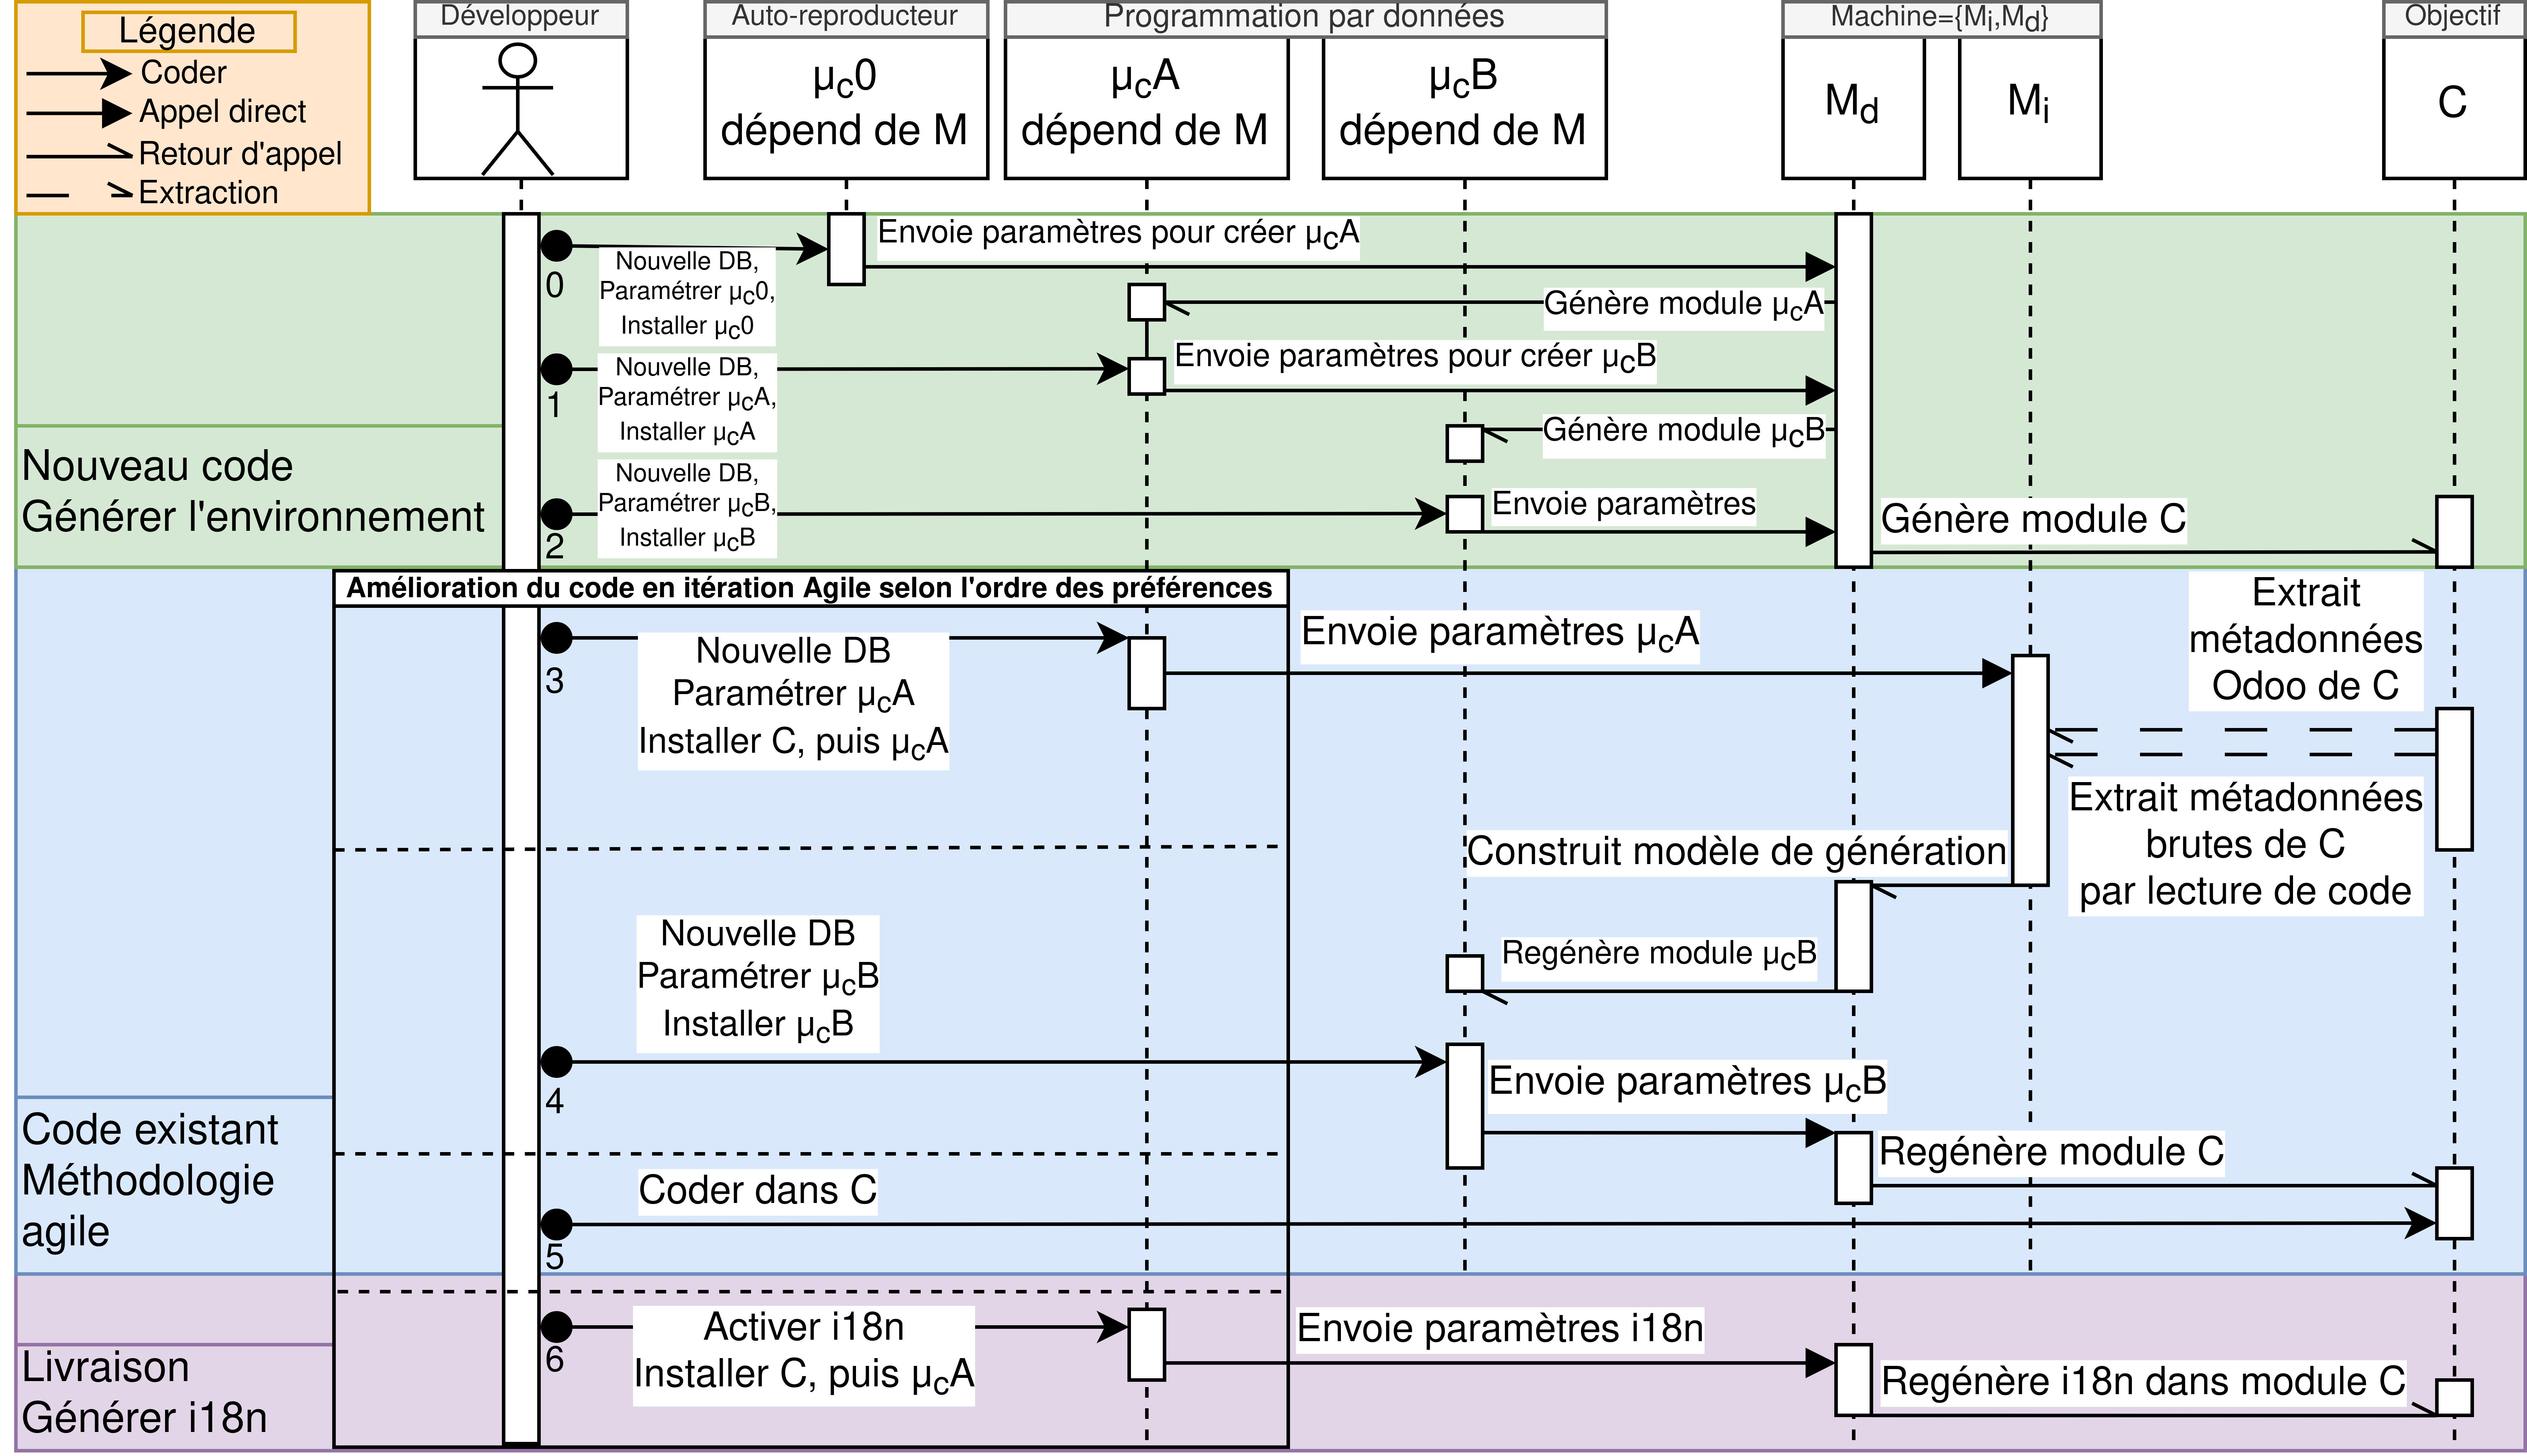
\includegraphics[width=6.535in]{images/code_generateur_erplibre_global_sequence.drawio.png}
\caption{Interaction du développeur avec le générateur de code}
\label{fig:dia_sequence_gc}
\end{figure}

Au départ d’un nouveau module code, µ$_C^0$ génère µ$_C^A$ qui génère µ$_C^B$ qui génère C. Il existe un script qui automatise un nouveau code, le développeur peut paramétrer le nom des modules et leurs emplacements. Ensuite, le développement commence en itération agile, les actions de 3 à 6 peuvent être exécutées dans l’ordre du choix du développeur.

% TODO expliquer raison/avantage de modifier soit µ$_C^A$, µ$_C^B$ ou le code directement.

Passer par l’étape 3 permet de mettre à jour l’étape 4 selon l’état du code via la rétro-ingénierie. Passer par l’étape 4 permet de mettre à jour le code selon le générateur. Il est possible de générer de nouvelles sections, comme la vue portail. Passer à l’étape 5 permet de personnaliser le code directement. Passer par l’étape 6 permet de mettre à jour le i18n de manière automatique.

La livraison sert à générer le i18n. C’est Odoo qui le génère, mais le générateur envoie les commandes, la liste des langues désirées à supporter et place les fichiers aux bons endroits dans le module. La raison pour laquelle c’est µ$_C^A$ qui doit le générer, c’est parce que le module doit être fini d’être généré et rechargé pour ensuite générer les langues, sinon ils sont corrompus par les traces de µ$_C^B$.

% TODO mettre dans discussion : Dans un contexte où l’ingénierie et la rétro-ingénierie serait parfaite, on n’aura pas besoin de mémoriser µ$_C^A$ et µ$_C^B$. Entre-temps, il y a une intervention humaine sur chacun de ces modules pour accélérer le développement. L’outil Git est utilisé pour faire des comparaisons entre les états d’itérations, seul ce qui est commité contient le bon contenu.

\subsection{Architecture}

La figure~\ref{fig:dia_architecture_automate}, elle démontre un développeur qui utilise l'interface de la machine qui opère dans le noyau de la machine.

\begin{figure}[htb]
\centering
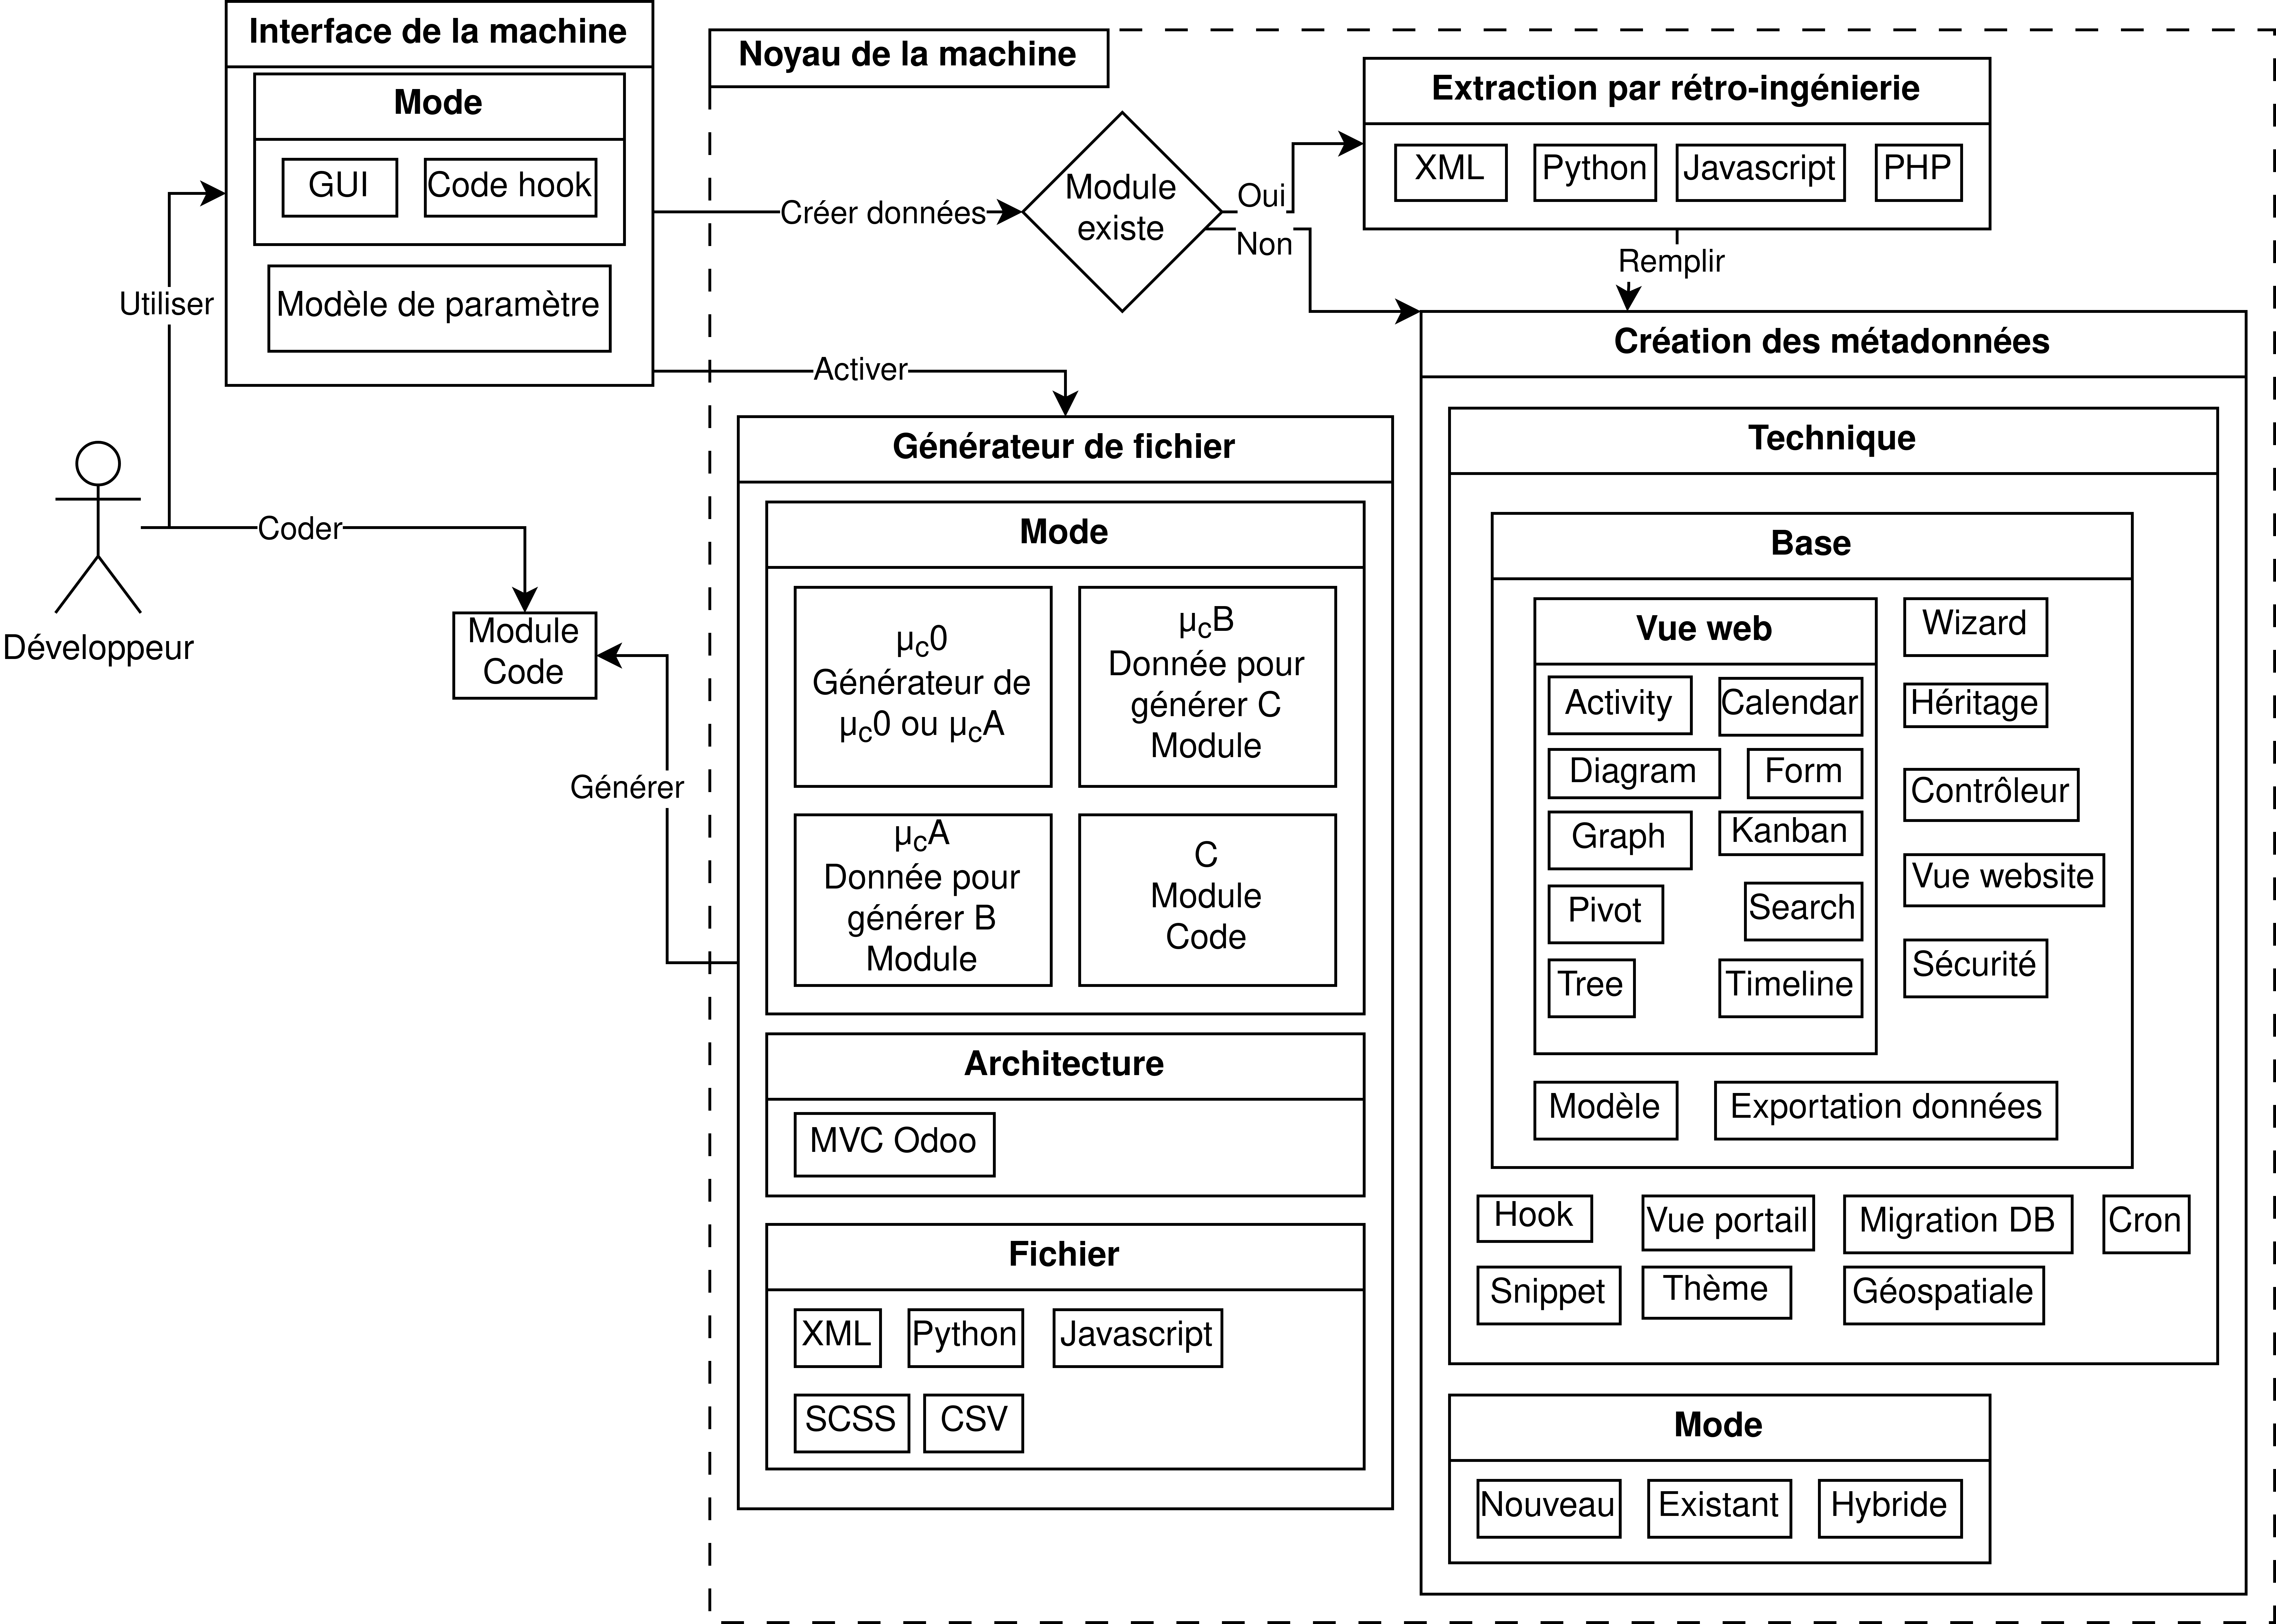
\includegraphics[width=6.535in]{images/architecture_machine.drawio.png}
\caption{Architecture de l'automate}
\label{fig:dia_architecture_automate}
\end{figure}

\begin{enumerate}
    \item L’interface machine permet à l’utilisateur de créer un modèle de données pour indiquer à la machine quelle opération effectuée avec leurs données associées. Plusieurs combinaisons, héritables, sont possibles selon les différentes techniques. De plus, c’est ici qu’on vient activer la génération de code.
    \item L’extraction par rétro-ingénierie permet de remplir le modèle de méta-données sans passer par la paramétrisation. Il extrait des informations qui ne sont pas accessibles dans le modèle de données d’Odoo sur le module.
    \item La création de méta-données se fait soit par l’utilisateur via la GUI ou le «Code Hook», il gère à la fois plusieurs techniques qui sont dans des modules. Le mode «nouveau» permet de créer de nouvelles données. Une fois qu’ils sont créés, c’est le mode «existant» qui est utilisé. Cependant le mode «hybride» permet d’écraser les données existantes en réactivant le mode «nouveau».
    \item Le générateur de fichier se fait activer par l’interface, mais il prend les méta-données pour faire sa génération selon le mode qu’il doit générer et l’architecture qu’il connaît. Il fait des liaisons entre les modèles et les vues en référence aux noms des champs de chaque modèle de données.
\end{enumerate}

Chacun de ces blocs de l’architecture est modulaire, chaque technique est héritable pour modifier le comportement et ajouter des liaisons pour permettre une génération de code au final.

La sécurité dépend du modèle. Le contrôleur dépend du modèle. La vue dépend du contrôleur et du modèle.

\subsection{Auto-générateur}

Représenté par µ$_C^0$, c’est un auto-générateur! Au moment de son installation, il génère le même code que lui-même au même endroit dans le système de fichier. Une légère modification va créer une autre entité qui sera une déviation dans l’objectif de démarrer une chaîne.

C'est le module \texttt{M} qui contient les méta-données de µ$_C^0$. Ainsi, exécuter µ$_C^0$ devient un test de fonctionnalité et c'est un succès lorsqu'il n'y a pas de différence. Cependant sa programmation est actuellement spécifique à sa génération, aucun autre module n’a besoin de cette fonctionnalité unique.

% TODO TODO calcul code unique. HOW. Regarder le nombre de ligne exécuter avec ce module VS le nombre de ligne pour un autre module simple même type -> son µ$_C^A$ avec aucun modèle et un hook.
% TODO mettre référence vers le code

% Il pourrait être plus petit, faire appel à des méthodes extérieures. De plus, il pourrait y avoir moins de paramètre, on est pris entre la faciliter de paramétrer rapidement et la gestion de la lourdeur de beaucoup de paramètres. Présentement, la machine est limitée en fonctionnalité, mais plus que ça va avancer, plus il y aura de paramètres et il en aura trop pour tous les ajouter.

% TODO le terme chaine est nouveau, il faudrait le définir

L'auto-générateur est utilisé pour générer des µ$_C^A$ avec une légère modification dans les paramètres. Même s'il a la capacité de générer un µ$_C^B$, mieux vaut créer la chaîne proposé pour faire de l'amélioration continue.

\section{Résultats propres à SO-1}

\subsection{Génération par gabarit}

La génération par gabarit était déjà supportée dans la version initiale~\cite{bluiksnot_repo}, de plus, il y a eu des améliorations :
\begin{enumerate}
%TODO mettre en référence \footnote{\url{https://docs.python.org/3/whatsnew/3.6.html#pep-498-formatted-string-literals}}
    \item Utilisation des f-strings au lieu d'utiliser la fonction «format» de String.
    \item Utilisation de la bibliothèque Code-writer en Python\footnote{\url{https://pypi.org/project/code-writer/}}
    \item Utilisation de la bibliothèque lxml\footnote{\url{https://pypi.org/project/lxml/}}
\end{enumerate}

\subsection{MVC}

L’architecture MVC était déjà supportée dans la version initiale~\cite{bluiksnot_repo}, de plus, il y a eu des améliorations : 

\begin{enumerate}
% TODO define Wizard
 \item Ajout de bouton qui ouvre des «Wizard» pour générer les «Views», les «Models» et les «Controllers». Ainsi le développeur peut les configurer et demander de générer les méta-données associées.
\begin{figure}[htb]
\centering
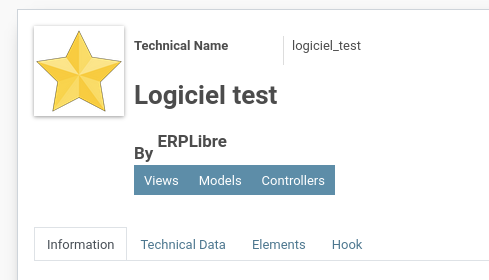
\includegraphics[width=3in]{images/GUI_MVC.png}
\caption{Architecture de l'automate}
\label{fig:dia_gui_mvc}
\end{figure}
 \item Les règles de sécurité sont ajustées selon les configurations et personnalisables par la suite.
\end{enumerate}

\subsection{Générer un module à partir d’une base de données externes}

% Un module a été programmé pour suivre la technologie ETL
% TODO manque le load de https://fr.wikipedia.org/wiki/Extract-transform-load
% ça devient discussion

La migration de données à partir de \texttt{SQL} était déjà supporté dans la version initiale, cependant il y a eu des améliorations : 

\begin{enumerate}
    \item Ajout de type de données, dont ceux utilisé par le projet Accorderie
    \item Ajout d'association entre les types de données et les différentes personnalisations de l’architecture Odoo
    \item Interface représentant la base de données avec les contrôleurs permettant la configuration de la migration sur le modèle de données désirés
    \item Gestion des interdépendances (A de B et B de A)
\end{enumerate}

\subsection{Génération de code par des données}

La capacité de prendre les données via les interfaces utilisateurs telles que la GUI et le «Code hook» est de la génération de code par des données. Cela permet de personnaliser pour obtenir un logiciel adapté à ce que l’utilisateur est capable d’exprimer.

L’automate est une machine qui grâce à son interface «code hook», il se fait commander par deux couches de méta-données paramétrable par l’humain. Les deux couches s’interfèrent entre eux pour permettre l’évolution de la fonctionnalité désirée.

% TODO diagramme de couche entrée de l’utilisateur et sortie des fonctionnalités.

\section{Résultats propres à SO-2}

\subsection {Extraction de code et reproduction}

De la macro et micro extraction a été réalisé avec plusieurs techniques combinées.

Pour pouvoir faire de la reproduction, il a suffit de faire de la macro extraction, c'est-à -dire faire une recherche dans toutes les classes pour copier le contenu de chaque méthode pour le transformer en méta-données et pouvoir faire l’opération direct de générer le code qui a été copié. L’utilisation de l’\texttt{AST} a servi à déterminer quelle ligne de code était à découper pour les recopier.

Cependant il était nécessaire dans certain contexte de faire de la micro extraction, comme : 
\begin{enumerate}
    \item L’extraction des noms des constantes, ils sont transformés en valeur lors de l’exécution;
    \item L’extraction des commentaires, qui n’est pas supporté dans la bibliothèque \texttt{AST} de Python 3.7;
    \item L’extraction des décorateurs;
    \item L’extraction des paramètres et nom des méthodes/fonctions;
    \item Les méta-informations d’un modèle (description, nom, etc.)
\end{enumerate}

De plus, les vues ont été extraites dans le but d'obtenir des méta-données spécifiques qui caractérise la reconstruction de la vue, ces données n’étaient pas accessibles dans les données d'Odoo.

Certaines informations ont été extraites dans le Javascript à l’aide de la bibliothèque «pyjsparser».

Pour l’extraction d'un projet externe d'une autre technologie, un extracteur de PHP a été développé via un «parser» de la communauté\footnote{\url{https://github.com/JameelNabbo/PHP-Parsers}}.

% TODO manque info sur le générateur de générateur de code
C'est en développent les techniques de génération de code qu'on réalise la reproduction. Un script a été développé pour accélérer l’écriture du générateur de code, ainsi un générateur de générateur de code. Ensuite le développeur peut le transformer légèrement pour prendre les paramètres des méta-données.

\subsection {Amélioration continue sur la génération}

Grâce à l’extraction des méta-données, dès que la technique de génération est bien développé avec les méta-données, le code est automatiquement généré avec des bonnes pratiques logicielles corrigeant automatiquement les problèmes.

L’intérêt de passer par Odoo pour lire le module valide déjà certains fonctionnements (par exemple : pas d’erreur de syntaxe dans le Python ou les \texttt{XML} étaient bien construits).

Ainsi, pour un module désiré, nous utilisons les outils pour générer µ$_C^A$ et µ$_C^B$, puis en avançant dans le développement, nous bouclons entre le 3 et 4 sur Figure~\ref{fig:dia_sequence_gc}.

\subsection {Test de validation de génération de codes}

Pour tester ce générateur de code, la technique du test de comparaisons des sorties de la génération a été utilisé. Pour procéder, un développeur valide via l'outil Git ce qui est commité\footnote{Un terme dans l'outil Git pour valider le code en créant un état dans l'historique.}. Ainsi, un script a été développé pour lancer en parallèle les tests et valider les différences de génération avec ce qui a été commité précédemment. Aucune différence est un succès.

Il y a plusieurs types de test : 
\begin{enumerate}
    \item Valider l’installation du module généré;
    \item Valider que µ$_C^B$ génère bien le module cible sans différence dans le code;
    \item Valider que µ$_C^A$ génère bien µ$_C^B$ sans différence dans le code;
    \item L’extraction des paramètres et nom des méthodes/fonctions;
    \item Valider que la migration d’une base de données \texttt{SQL} se fait sans différence dans le code.
\end{enumerate}

En exécutant tous les tests, voir annexe~\ref{annexe_test_generateur_code}, une couverture de 84\% est obtenu, tous les tests présents sont un succès, sauf ceux sur l’auto-générateur.

\subsection {Règles de codage standardisées}

Au moment de générer les fichiers, toutes les sorties textes sont traitées par des outils de mise en forme suivant des règles de codage standardisées.

Pour le Python, l’outil «black» est utilisé pour la mise en forme, suivant le standard \texttt{PEP8} avec «isort» pour réordonner les importations. «black» donne une mise en forme non naturel comparé à l’écriture de code pour un humain, cependant son résultat facilite la lecture et le suivi des différences pour les futurs ajouts.

Le Javascript, le HTML et le \texttt{XML} sont mises en forme avec l’outil «prettier».

De plus, le générateur force le déplacement des classes dans leur propre fichier respectif pour faire une classe par fichier.

Les champs pour chaque modèle sont déplacés en ordre alphabétique, mais le premier est celui qui est utilisé pour représenter le modèle\footnote{Référence à l'attribut «\_rec\_name»}.
